\documentclass[12pt,a4paper]{article}
\usepackage[T1]{fontenc}
\usepackage[utf8]{inputenc}
\usepackage{mathptmx}
\usepackage[margin=1in]{geometry}
\usepackage{setspace}
\usepackage{graphicx}
\usepackage{booktabs}
\usepackage{amsmath}
\usepackage{enumitem}
\usepackage{tikz}
\usetikzlibrary{positioning,arrows.meta,calc}
\usepackage[font=small,labelfont=bf,skip=3pt]{caption}
\usepackage[hidelinks]{hyperref}
\onehalfspacing
\setlist{nosep,leftmargin=1.4em}
\newcommand{\code}[1]{\texttt{\small #1}}
\newcommand{\tbd}[1]{\textbf{[#1]}}
\renewcommand{\abstractname}{}
\usepackage{titlesec}
\titleformat{\section}{\bfseries\normalsize}{\thesection.}{0.5em}{}
\titleformat{\subsection}{\bfseries\normalsize}{\thesubsection}{0.5em}{}
\titlespacing*{\section}{0pt}{6pt}{0pt}
\titlespacing*{\subsection}{0pt}{3pt}{0pt}

\begin{document}
\begin{center}
{\bfseries\Large Third Eye: A Phone-Based Referee for Physical Jenga Using LiDAR Depth, Fiducial Pose and Compiled Rulebooks}\\[4pt]
\singlespacing
Aadit Pani (1RVU23CSE002), Mitul KM (1RVU23CSE273), Megh Mavani (1RVU23CSE260)\\
School of Computer Science and Engineering, RV University, Bengaluru, India\\
\tbd{email addresses} $|$ Guide: \tbd{faculty name} $|$ Team No.\ \tbd{team number}
\end{center}
\onehalfspacing

\noindent\textbf{Abstract---}Refereeing a physical game needs the position of every piece and a rulebook. We present Third Eye, a system that watches a Jenga tower with an iPhone (LiDAR) and an optional Android phone, marks which blocks may legally and safely be pulled, names the block that was pulled, and calls a collapse. The work is an engineering study of the system as built: ArUco markers on a calibrated board place the tower in a fixed frame, a LiDAR box fit and an edge-snapping step keep the overlay on the tower, a colour-based finder compares end faces before and after each move, and a compiled rulebook with a balance model decides what is legal. On three recorded games (1{,}706 saved frames) frames arrive at 2.85--3.00\,Hz. On 31 pulls with a known layer the finder is right for 77\,\% of pulls (94\,\% within one layer); a calibrated confidence of at least 90\,\% adds a block automatically and the player answers Yes or No. The finder needs 0.2--0.3\,s of computation per move on a Mac. In three replayed games the collapse detector flagged the one real fall and raised no false alarm. The data are small and the rules were tuned on them, so none of the figures is held out.\\[2pt]
\noindent\textbf{Keywords---}Jenga, LiDAR, ArUco, physical-game refereeing, pose estimation, rule checking

\section{Introduction}
A referee for a physical game must know the state of the pieces and apply the rules. For Jenga the state is a stack of $L$ layers of three blocks; the rules say which block may be pulled and when the game ends. Third Eye names the pulled block and flags illegal or dangerous pulls using commodity phones and no special table.

Contributions of this work:
\begin{itemize}
\item a phone-only rig with an overlay fixed to a calibrated marker board, a LiDAR correction and edge-snapping;
\item a colour-based pull finder with calibrated confidence (Yes or No above 90\,\%);
\item a guarded collapse detector and a rule checker driven by a compiled rulebook;
\item a working prototype (live 3D tower, replay, wired mode) and an honest evaluation on small data.
\end{itemize}

\section{Related Work}
Fazeli et al.\ learn a hierarchical model that fuses force and vision so a robot can extract Jenga blocks without toppling the tower~\cite{fazeli}; their task is manipulation with a force-sensing wrist, ours is observing a human game. Assembly101 provides multi-view video of procedural activity and a mistake-detection task~\cite{sener}, and a survey covers augmented-reality guidance for assembly~\cite{wang}; both rely on learned recognition or guidance rather than explicit rules. Fiducial markers~\cite{garrido} give camera pose. Phone LiDAR is accurate to about $\pm1$\,cm~\cite{luetz}, coarse next to 15\,mm layers, and dense fusion such as KinectFusion~\cite{newcombe} needs finer surfaces than ARKit meshes give. Hand detection uses MediaPipe Hands~\cite{mediapipe}. We calibrate cameras after Zhang~\cite{zhang}, solve the marker board by bundle adjustment~\cite{triggs}, fit the tower with Geman--McClure robust weights~\cite{geman}, and an early finder used phase correlation~\cite{kuglin}.

\begin{table}[h]
\centering\small\singlespacing
\caption{Summary of related work.}\label{tab:rel}
\begin{tabular}{@{}p{0.5cm}p{3.1cm}p{3.3cm}p{3.6cm}p{2.7cm}@{}}
\toprule
Ref. & Method / model & Data & Result & Limitation \\
\midrule
\cite{fazeli} & hierarchical vision + force policy & robot Jenga trials & extracts blocks & needs force sensing \\
\cite{sener} & multi-view video benchmark & 4{,}321 videos, toy assembly & recognition, mistakes & learned, no explicit rules \\
\cite{garrido} & ArUco fiducials & synthetic, real & robust pose & markers must be visible \\
\cite{luetz} & iPhone 12 Pro LiDAR study & geoscience objects & $\approx\pm1$\,cm & coarse for 15\,mm \\
\textbf{Ours} & marker pose, LiDAR fit, colour finder, rules & 3 + 10 recorded games & 77\,\% pull layer, 1/1 fall & small, tuned on same data \\
\bottomrule
\end{tabular}
\end{table}
Table~\ref{tab:rel} summarises the closest work. The gap we address is the integration: a phone-only referee in which the player's confirmation is trusted over noisy depth and a compiled rulebook decides legality. We make no claim of superiority over any cited system.

\section{Problem Formulation}
Let the tower have $L$ layers with three slots $s\in\{0,1,2\}$ and occupancy $o_{\ell s}\in\{0,1\}$. A move removes one block $(\ell,s)$ and places it on top. Given images $I_t^c$ from cameras $c$, depth $D_t$ and the player's MARK tap, the system outputs (a) the pulled block $(\ell,s)$, (b) for every standing block whether pulling it is allowed and stable, and (c) a game-over signal.

\section{Dataset}
\subsection{Data source and description}
There is no public dataset for this task, so we recorded our own. The iPhone saves, every 20th ARKit frame, a $1920\times1440$ JPEG, a $256\times192$ depth map with confidence, intrinsics and pose; the Android phone saves $1280\times720$ JPEGs. Acquisition statistics come from three recorded iPhone games (647, 496 and 563 frames, 1{,}706 in all, none missing a file). Pull labels come from 10 recorded sessions (31 pulls with a known layer): the layer is known if the player typed a correction, or if the finder was confident and was not corrected.
\subsection{Preprocessing and split}
End-face crops are $32\times32$ normalised grayscale; depth keeps confidence-2 pixels between 0.05 and 1.5\,m. Nothing is trained, so there is no split; the constants (confidence tiers, thresholds) were chosen on these same sessions, so the figures are \emph{not} held out.

\section{Proposed Methodology}
\subsection{System architecture}
\begin{figure}[h]
\centering\small
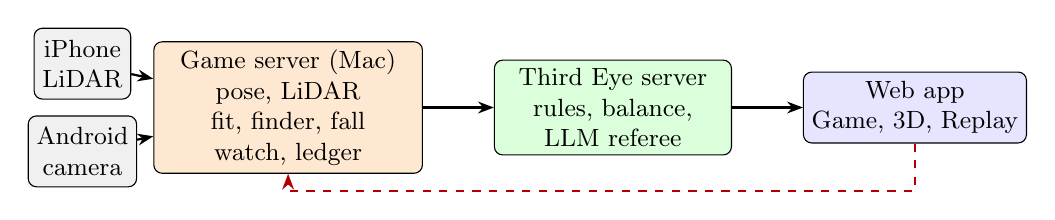
\begin{tikzpicture}[font=\small, node distance=6mm,
  b/.style={draw, rounded corners=3pt, align=center, minimum height=9mm, inner sep=3pt, fill=gray!12},
  a/.style={-{Stealth[length=2mm]}, thick}]
\node[b] (ip) {iPhone\\LiDAR};
\node[b, below=2mm of ip] (an) {Android\\camera};
\node[b, right=9mm of $(ip)!0.5!(an)$, fill=orange!18, text width=3.2cm] (gs) {Game server (Mac)\\pose, LiDAR fit, finder, fall watch, ledger};
\node[b, right=9mm of gs, fill=green!14, text width=2.8cm] (te) {Third Eye server\\rules, balance, LLM referee};
\node[b, right=9mm of te, fill=blue!10] (ui) {Web app\\Game, 3D, Replay};
\draw[a] (ip) -- (gs); \draw[a] (an) -- (gs); \draw[a] (gs) -- (te); \draw[a] (te) -- (ui);
\draw[a, dashed, red!70!black] (ui.south) -- ++(0,-6mm) -| (gs.south);
\end{tikzpicture}
\caption{Architecture. Solid: data. Dashed: player commands (MARK, Yes/No, typed move).}\label{fig:arch}
\end{figure}
Figure~\ref{fig:arch} shows the pipeline. The phones post frames over Wi-Fi or a USB cable. The game server computes pose, fit, finder and fall watch, keeps the ledger of confirmed pulls and sends the browser a raw JPEG plus overlay shapes; the Third Eye server follows the ledger, evaluates the rules and serves the interface.
\subsection{Model description}
\textbf{Pose and overlay.} Four 40\,mm ArUco markers (DICT\_4X4\_50) on a fixed board give the tower pose by \code{solvePnP}. Their layout is solved once by bundle adjustment, so every game starts calibrated. For the iPhone, depth is back-projected, $X=(u-c_x)d/f_x$, $Y=(v-c_y)d/f_y$, $Z=d$, and a 7-parameter box fit (shift, rotation, height) with Geman--McClure weights corrects the pose; this correction must not be applied to the Android camera, whose overlay otherwise sat one layer too high. For each camera, edge-snapping nudges the projected outline onto the tower's image edges; poses are smoothed (EMA $\alpha=0.2$).

\textbf{Pull finder.} After MARK, the finder takes a calm window before and after the move (found from hand and motion activity) and compares, for each layer $\ell$ and camera $c$, the median face crops: $d_{c\ell}=\lVert \tilde a_{c\ell}-\tilde b_{c\ell}\rVert_1/1024$, z-scored per camera and summed, $s_\ell=\sum_c (d_{c\ell}-\mu_c)/\sigma_c$. The winning score and its gap to the runner-up map to a calibrated confidence. At $\ge90\,\%$ the block is added and the player answers Yes or No; below that the player types the move.

\textbf{Rules and collapse.} A pull is allowed if the layer is not the bottom or the top complete layer and, after the pull, the centre of mass above every layer stays inside the footprint of its remaining blocks with a 4\,mm margin. Pulled blocks go back on top. A fall needs a height watch and a point-cloud standing check, each corroborated by a $\ge30$\,mm drop of the 95th-percentile height, with a guard for a hand over the lens; false alarms clear themselves.
\subsection{LLM component and training details}
A hosted language model compiles a natural-language rulebook into a validated spec and answers questions (``Which blocks can I still take safely?'') from the checker's verdict, citing the rules; it never sees video and nothing is fine-tuned (15 of 16 rulebooks compiled with a 120B hosted model, 7 of 16 with an 8B local one). No neural network is trained; the parameters are fixed: 15\,mm layers, 4\,mm balance margin, EMA 0.2, confidence tiers (typed 92/89/85/82\,\%, free 95/91/88/84\,\%), auto-apply at 90\,\%, a 1.6\,s calm window and a 30\,mm fall drop.

\section{Prototype and Deployment}
\subsection{Prototype description (UI/UX)}
The web app has three screens. \textbf{Game} shows both camera feeds with the green (may be pulled), amber (loose) and red (not allowed) overlay (Fig.~\ref{fig:ui}a) and every control: record, MARK, Yes/No, typed move, tower settings, re-detect, overlay lock, rotate view and New game. \textbf{3D tower} carries the same controls beside a live 3D tower: on Yes the block comes off the model in about half a second. \textbf{Replay} (Fig.~\ref{fig:ui}b) rebuilds any recorded game move by move with a 3D scrubber and the before/after crops; a banner shows when judging is paused for a hand.
\begin{figure}[t]
\centering\singlespacing
\includegraphics[height=4.6cm]{fig_overlay.png}\hspace{1cm}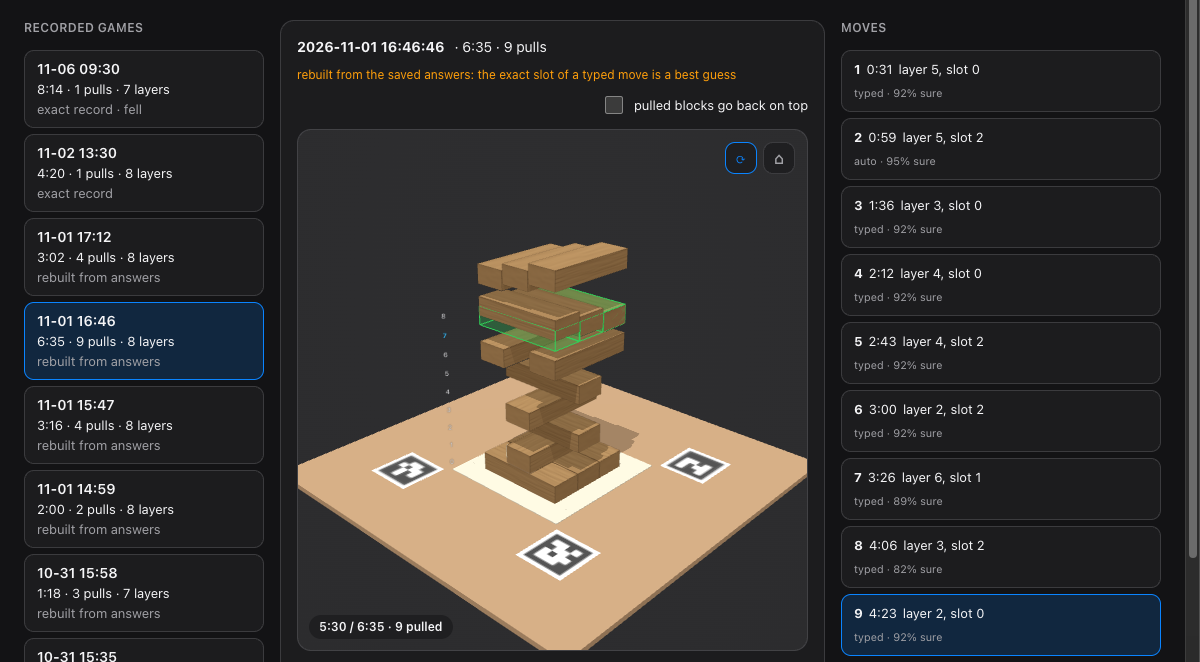
\includegraphics[height=4.6cm]{fig_replay.png}
\caption{(a) Overlay on the iPhone view; layers are counted from the bottom. (b) Replay of a recorded 8-layer game: the 3D tower after nine pulls, and the move list with confidence.}\label{fig:ui}
\end{figure}
\subsection{Deployment details}
Third Eye is a local demo, not a hosted service: two Python servers run on a Mac (game server on port 8000, Third Eye on 8001, started by \code{scripts/start\_all.sh}) and the browser runs on the same Mac. Phones connect over Wi-Fi or a USB cable (the iPhone queues requests that a bridge on the Mac collects; the Android uses \code{adb reverse}). \tbd{Public URL: none; local demo only}.
\subsection{GitHub repository}
Repository: \url{https://github.com/switchtwitch12345/third-eye-testing} \tbd{confirm it is public; add licence}. It holds the game server and finder (\code{iphone\_saved.py}, \code{move\_infer.py}), pose, fit and edge code (\code{tower\_*.py}), rules and tests (\code{jenga\_rules.py}), the iPhone and Android apps, and \code{scripts/} and \code{patches/} for wired mode and the UI.

\section{Experimental Setup}
\subsection{Implementation environment}
Stage timings use single-threaded OpenCV and Python 3.13 on an AMD Ryzen 5 5600H laptop; replays of the current server ran on the game Mac, calling its own functions on recorded frames, so they exclude network and the player's hand time.
\subsection{Metrics and baselines}
Finder: exact accuracy, accuracy within one layer and the share of moves reaching 90\,\%. Collapse: true detections and false alarms per game. Cost: median time per stage. The finder is compared across iPhone-only, Android-only and combined cameras, and against depth-only pull detection (repository notes).

\section{Results and Analysis}
\textbf{Acquisition.} Saved-frame spacing is 333\,ms in all three games ($60/20$\,Hz); rates are 3.00, 2.91 and 2.85\,Hz (two gaps of 5.2 and 3.6\,s); a frame costs 0.78--0.87\,MB.

\textbf{Finder.} Table~\ref{tab:find} gives accuracy on the 31 known pulls. The best combination (81\,\%) was chosen after seeing the data and is not held out. Replayed through the current server, all 5 moves of one 8-layer game reached 95\,\% and were applied automatically; in another, 6 of 10 did and 4 stayed near 50\,\% and were typed. Older games recorded before board calibration failed (no move reached 90\,\%), so the finder depends on the calibrated board. Depth alone found 3 of 10 pulls with corrective options and 0 without.
\begin{table}[h]
\centering\small\singlespacing
\caption{Layer accuracy on 31 labelled pulls (uncorrected confident answers counted as right).}\label{tab:find}
\begin{tabular}{@{}lrrr@{}}
\toprule
Method & Exact & Within 1 layer & n \\
\midrule
iPhone only & 79\,\% & 93\,\% & 29 \\
Android only & 53\,\% & 90\,\% & 30 \\
Both cameras (mean) & 77\,\% & 94\,\% & 31 \\
Both, product rule & 81\,\% & 94\,\% & 31 \\
Depth only (1 camera) & 0--30\,\% & -- & 10 \\
\bottomrule
\end{tabular}
\end{table}

\textbf{Time and cost.} The finder computes in 0.18--0.34\,s per move on the Mac; the calm window it waits for is at least 1.6\,s (4.5\,s earlier), so the player sees about 2\,s plus polling. This speed-up is derived from the settings, not measured as a before/after. On the laptop the box fit costs 62.2\,ms (median), pose solve 10.8\,ms, ArUco at 960\,px 7.1\,ms; the full pipeline replays at 24--28\,ms per frame, 8--10$\times$ faster than real time, and the rule checker scales as $L^3$ (slope 2.80).

\textbf{Overlay and fall.} On five Android frames edge-snapping moved the pose by at most 2.4\,mm and 0.8$^\circ$ and about doubled our own edge-alignment score (not a position error). Replaying depth from three games, the one fall was declared at 381\,s and the other two games raised no false alarm.

\section{Discussion}
The colour finder works because a pulled block changes the look of one end face, and combining both cameras guards against one bad view; the iPhone is stronger than the Android alone. Failures concentrate where hands or shadows change the faces, so below 90\,\% the player types the move. Depth is too noisy for the pull itself (a 15--35\,mm dent) but good for height and collapse. Each fall guard comes from a real failure (a hand over the lens, a collapsing fitted height, an empty cloud). Limitations: three games and 31 pulls, one tower and one iPhone; optimistic labels; rules tuned on the same sessions; wired-versus-Wi-Fi rate, end-to-end latency and hand detection were not measured.

\section{Ethical Considerations and Responsible AI}
The cameras film hands and rooms, so recordings stay local and out of the repository; the participants were the authors. The system only advises a game, and below 90\,\% it asks the player. The language model receives the checker's text, not video. ArUco, OpenCV and MediaPipe are used under open licences.

\section{Conclusion and Future Work}
Third Eye shows that two phones, markers on a calibrated board and a compiled rulebook can referee a Jenga game: the overlay stays on the tower, the finder names the pulled layer correctly for about four in five pulls and asks the player when unsure, and the fall detector flagged the one real collapse without false alarms. Future work: overlay error against hand-labelled corners, a held-out finder test on new games with independent ground truth, a measured time from MARK to the answer, wired-versus-Wi-Fi frame rates, and more recorded falls.

\section*{Acknowledgment}
We thank our guide \tbd{faculty name} and the School of Computer Science and Engineering. AI-tool disclosure: an AI assistant (Claude, Anthropic) helped write code and draft this paper; the authors ran the experiments and checked the results.

\begin{thebibliography}{99}\footnotesize\singlespacing\setlength{\itemsep}{0pt}
\bibitem{fazeli} N. Fazeli et al., ``See, feel, act: Hierarchical learning for complex manipulation skills with multisensory fusion,'' \emph{Science Robotics}, vol. 4, no. 26, 2019.
\bibitem{sener} F. Sener et al., ``Assembly101: A large-scale multi-view video dataset for understanding procedural activities,'' in \emph{Proc. IEEE/CVF CVPR}, 2022.
\bibitem{wang} X. Wang, S. K. Ong, and A. Y. C. Nee, ``A comprehensive survey of augmented reality assembly research,'' \emph{Advances in Manufacturing}, vol. 4, no. 1, pp. 1--22, 2016.
\bibitem{garrido} S. Garrido-Jurado et al., ``Automatic generation and detection of highly reliable fiducial markers under occlusion,'' \emph{Pattern Recognition}, vol. 47, no. 6, pp. 2280--2292, 2014.
\bibitem{luetz} G. Luetzenburg, A. Kroon, and A. A. Bj\o rk, ``Evaluation of the Apple iPhone 12 Pro LiDAR for an application in geosciences,'' \emph{Scientific Reports}, vol. 11, 2021.
\bibitem{newcombe} R. A. Newcombe et al., ``KinectFusion: Real-time dense surface mapping and tracking,'' in \emph{Proc. IEEE ISMAR}, 2011, pp. 127--136.
\bibitem{mediapipe} F. Zhang et al., ``MediaPipe Hands: On-device real-time hand tracking,'' arXiv:2006.10214, 2020.
\bibitem{zhang} Z. Zhang, ``A flexible new technique for camera calibration,'' \emph{IEEE Trans. Pattern Anal. Mach. Intell.}, vol. 22, no. 11, pp. 1330--1334, 2000.
\bibitem{triggs} B. Triggs et al., ``Bundle adjustment --- a modern synthesis,'' in \emph{Vision Algorithms: Theory and Practice}, 1999, pp. 298--372.
\bibitem{geman} S. Geman and D. E. McClure, ``Statistical methods for tomographic image reconstruction,'' \emph{Bull. Int. Statist. Inst.}, vol. 52, 1987, pp. 5--21.
\bibitem{kuglin} C. D. Kuglin and D. C. Hines, ``The phase correlation image alignment method,'' in \emph{Proc. IEEE Int. Conf. Cybernetics and Society}, 1975, pp. 163--165.
\end{thebibliography}
\end{document}
